\PassOptionsToPackage{AutoFakeBold}{xeCJK}
% 设置假粗体
\documentclass{ctexart}
\usepackage{amsfonts}
% 使用该包不会导致数学公式报错、mathbb等指令
\usepackage{indentfirst} %缩进
\usepackage{xeCJK}    %使用系统字体
\usepackage{bm}       %粗体
\usepackage{fancyhdr} %自定义页眉页脚
\pagestyle{plain}                   %不设置页眉页脚
%%%%%%%%%%%%%%%%%%%%%%%%%%%%%%%%%%%%%%%%%%%%%%%%%%%%%%%%%%%%%%%%
% 字体定义
%%%%%%%%%%%%%%%%%%%%%%%%%%%%%%%%%%%%%%%%%%%%%%%%%%%%%%%%%%%%%%%%
\setmainfont{Times New Roman}  %默认英文字体.serif是有衬线字体sans serif无衬线字体
\setmonofont{Consolas}
\setCJKmainfont[ItalicFont={楷体}, BoldFont={黑体}]{宋体}%衬线字体 缺省中文字体为
\setCJKsansfont{黑体}
\punctstyle{hangmobanjiao}
%-----------------------xeCJK下设置中文字体------------------------------%
\setCJKfamilyfont{song}{SimSun}                             %宋体 song
\newcommand{\song}{\CJKfamily{song}}
\setCJKfamilyfont{fs}{FangSong}                      %仿宋  fs
\newcommand{\fs}{\CJKfamily{fs}} 
\let\kaishu\relax                                    %重定义楷体,打开假粗体
\newCJKfontfamily\kaishu{KaiTi}[AutoFakeBold] 
%\setCJKfamilyfont{ktgb}{KaiTi_GB2312}                      %楷体 GB2312
%\newcommand{\ktgb}{\CJKfamily{ktgb}}
\setCJKfamilyfont{yh}{Microsoft YaHei}                    %微软雅黑 yh
\newcommand{\yh}{\CJKfamily{yh}}
\setCJKfamilyfont{hei}{SimHei}                              %黑体  hei
\newcommand{\hei}{\CJKfamily{hei}}
\setCJKfamilyfont{hwxk}{STXingkai}                                %华文行楷  hwxk
\newcommand{\hwxk}{\CJKfamily{hwxk}}
%------------------------------设置字体大小------------------------%
\newcommand{\chuhao}{\fontsize{42bp}{63bp}\selectfont}     %初号, 1.5倍行距
\newcommand{\xiaochuhao}{\fontsize{36bp}{36bp}\selectfont} %小初号,单倍行距
\newcommand{\yihao}{\fontsize{26bp}{39bp}\selectfont}        % 一号, 1.5 倍行距
\newcommand{\erhao}{\fontsize{22bp}{33bp}\selectfont}        % 二号, 1.5倍行距
\newcommand{\xiaoerhao}{\fontsize{18bp}{18bp}\selectfont}       % 小二, 单倍行距
\newcommand{\sanhao}{\fontsize{16bp}{24bp}\selectfont}       % 三号, 1.5倍行距
\newcommand{\xiaosanhao}{\fontsize{15bp}{22bp}\selectfont}      % 小三, 1.5倍行距
\newcommand{\sihao}{\fontsize{14bp}{21bp}\selectfont}        % 四号, 1.5 倍行距
\newcommand{\banxiaosi}{\fontsize{13bp}{20bp}\selectfont}  % 半小四, 20pt行距
\newcommand{\xiaosihao}{\fontsize{12bp}{20bp}\selectfont}       % 小四, 20pt行距
\newcommand{\dawuhao}{\fontsize{11bp}{11bp}\selectfont}      % 大五号, 单倍行距
\newcommand{\wuhao}{\fontsize{10.5bp}{10.5bp}\selectfont}   % 五号, 单倍行距
\newcommand{\xiaowuhao}{\fontsize{9bp}{9bp}\selectfont}   %小五号,单倍行距
% 这里是导言区

\CTEXsetup[format={\bfseries\song\xiaosihao},aftername={\quad},indent={0bp},beforeskip={6bp},afterskip={6bp},format+={\flushleft}]{section}
\CTEXsetup[format={\bfseries\song\wuhao},aftername={\quad},indent={0bp},beforeskip={6bp},afterskip={6bp},format+={\flushleft}]{subsection}
\CTEXsetup[format={\bfseries\song\wuhao},aftername={\quad},indent={0bp},beforeskip={6bp},afterskip={6bp},format+={\flushleft}]{subsubsection}
\usepackage{ragged2e}
% 完善两端对齐部分
\usepackage{booktabs} 
%插入表格
\usepackage{graphicx}
% 插入图片
\usepackage{amsmath}
% 插入cases公式
\begin{document}

\begin{center}
    {\hei\sanhao 基于图嵌入技术的推荐算法研究}

    \vspace{1em}

    {\wuhao 廖雅璇\hspace{1em}李皓\hspace{1em}徐豪\hspace{1em}郑佳宇\hspace{1em}周洲}

    {\wuhao (电子科技大学,计算机科学与工程学院)}
\end{center}

% 中文摘要环境 
{\justifying\noindent
{\bfseries\song 摘\hspace{10bp}要:} 个性化推荐技术是当今互联网领域的热门研究领域,本项目构建了一种基于图嵌入式技术的推荐算法系统,用于帮助用户获取电影个性化推荐。该系统使用bootstrap与Django作为前后端框架,建立了用户友好的个性化推荐网页。该系统使用神经网络训练Scrapy获取的电影数据,最终为每个用户生成推荐结果,具有较好的应用前景。

\noindent\textbf{\bfseries\song 关键词:} 神经网络,Django,bootstrap,Scrapy}

\vspace{2em}

\begin{center}
    {\hei\sanhao Research on Recommendation Algorithm Based on Graph Embedding Technology}

    \vspace{1em}

    {\wuhao Yaxuan Liao\hspace{1em}Hao Li\hspace{1em}Hao Xu\hspace{1em}Jiayu Zhen\hspace{1em}Zhou Zhou}

    {\wuhao University of Electronic Science and Technology  }

    {\wuhao School of Computer Science and Engineering}

\end{center}
% 洋文摘要环境:todo设置洋文字体
{\justifying\noindent
{\bfseries\song Abstract:}Personalized recommendation technology is a hot research field in the Internet field. This project constructs a recommendation algorithm system based on graph embedded technology, which is used to help users to obtain personalized movie recommendations. The system uses bootstrap and Django as the front and back end framework to establish a user-friendly personalized recommendation web page. The system uses neural network to train the movie data obtained by Scrapy, and finally generates recommendation results for each user, which has a good application prospect.
 
\noindent\textbf{\bfseries\song Key Words: } Neural network , Django,bootstrap,Scrapy}
% todo:添加作者以及学院信息
% todo:更改标题的字号信息
% todo:英文相关的内容
\section{引言}
随着移动互联网的快速发展,我们进入了信息爆炸时代。当前通过互联网提供服务的平台越来越多,相应的提供的服务种类(购物,视频,新闻,音乐,社交等)层出不穷,为了更好的为用户提供服务,在为用户提供服务的同时赚取更多的利润,越来越多的公司通过采用个性化推荐技术,辅助用户更快地发现自己喜欢的东西。公司根据用户在产品上的行为记录,结合用户自身和物品的信息,利用推荐技术(机器学习的一个分支)来为用户推荐可能感兴趣的物品。推荐系统的主要思想是分析用户的历史行为和偏好进行建模,并自动向用户推荐感兴趣的物品,然后为用户获得个性化推荐列表。相比于传统的信息检索通过分类和搜索引擎去获取信息,推荐系统不需要用户提供明确的需求,甚至当用户自己都不明确自己的需求时,推荐系统通过分析用户的历史行为给用户建模,为用户推荐他感兴趣的物品或信息。

图嵌入是解决图分析问题的一种有效方法。图嵌入将图形数据转换为一个低维向量空间,在该空间中,图形结构信息和图形属性得到最大程度保留,图相关算法也能更简单地使用低维向量(嵌入)进行更有效率的计算。使用深度学习技术来进行图嵌入也是目前热门的研究领域,一些基于深度学习的图嵌入技术同时也属于图神经网络(Graph Neural Network, GNN),例如图卷积神经网络(Graph Convolutional Network, GCN)等。基于GNN的方法以其处理结构数据和探索结构信息的优势,已成为推荐系统中最新的方法。因此,基于图嵌入的推荐算法研究有着极大的研究意义。

\section{系统架构}
\subsection{网络后端}
本项目使用Django作为后端架构,其特点是注重应用开发的可重复性,以及“可插拔性”。该框架代码简洁,耦合度低,开发快速,国内外许多互联网企业都使用其作为产品的后端架构,如Instagram等。Django架构以模型为中心驱动网页开发,以url链接视图以及后端逻辑,易于进行前后端分离的系统设计。

\subsection{网络前端}
网络前端部分,我们使用了Bootstrap框架设计网页样式。我们前期共设计了五个页面,分别是登陆页面、注册页面、个人信息页面、未登录首页和登陆后首页。更多细节我们将在系统功能一节详细阐述。

\subsection{数据存储}
该项目采用MySQl系统作为数据存储数据库。MySQL在过去由于性能高、成本低、可靠性好,已经成为最流行的开源数据库,因此被广泛地应用在Internet上的中小型网站中。本项目中使用MySQl数据库存储了用户信息,以及电影类别信息等数据。其中用户信息含有用户名、密码、性别、注册日期、电影偏好等信息。电影数据库中维护电影名称,导演,演员,类别、评分、上映时间等字段。

\subsection{数据挖掘}
为了获得电影数据,系统使用Scrapy作为框架,在合理合法限度内对互联网资源进行搜集整理。截止目前,系统可提供的电影共575条。每部电影由电影图片、电影标题、电影类型、电影评分、电影剧情简介等元素组成。电影数据在豆瓣网爬取,总体来看采用通用爬虫和聚焦爬虫结合的方法。对目前的系统而言,电影数据量足以实现离线推荐功能。随着项目的推进,将尽可能实现基于Scrapy的分布式搭建,并在此基础上结合redis数据库实现增量式爬虫来获取更多的数据。

\section{系统功能}
该系统以网页形式呈现,因此依据各个视图介绍系统功能。

\subsection{未登录首页}
未登录首页是进入系统的第一个页面,页面左侧为电影分类;顶部有选择登录、注册功能和搜索栏,点击链接将分别进入登录页面或注册页面;首页主体则是电影图片、名称和上映时间,点击图片或名称将进入电影详情页面。在未登录时,首页的登录区域无用户名,主页的电影资源为根据网络热度得到的高分电影,并根据热度高低排序呈现。
\begin {figure}[h]
\centering % 居中显示
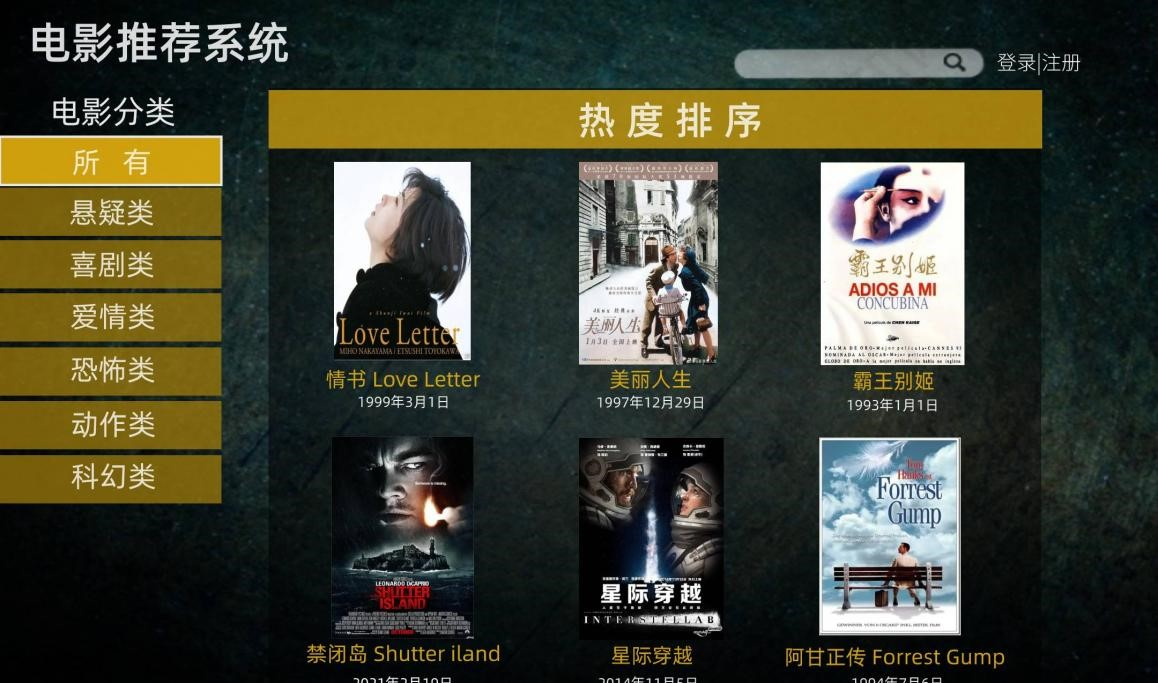
\includegraphics[width=\textwidth]{p1.jpg}
\caption{未登录首页样式} % 标题
\label{five}
\end {figure}

\subsection{登录页面}
点击首页的登录处将进入登录页面,顶部为“用户登录”的标题,页面主体为login表单,登录信息主要包括用户名、密码和验证码,验证码为随机图片,点击可切换。输入用户名和密码后,将输入的数据与后端数据库中的数据进行对比,同时比对验证码,用CSS和JS文件设置若均正确将进入登录后的主页页面,若任一不正确则提示错误,用户名不存在会提示注册账号。
\begin {figure}[h]
\centering % 居中显示
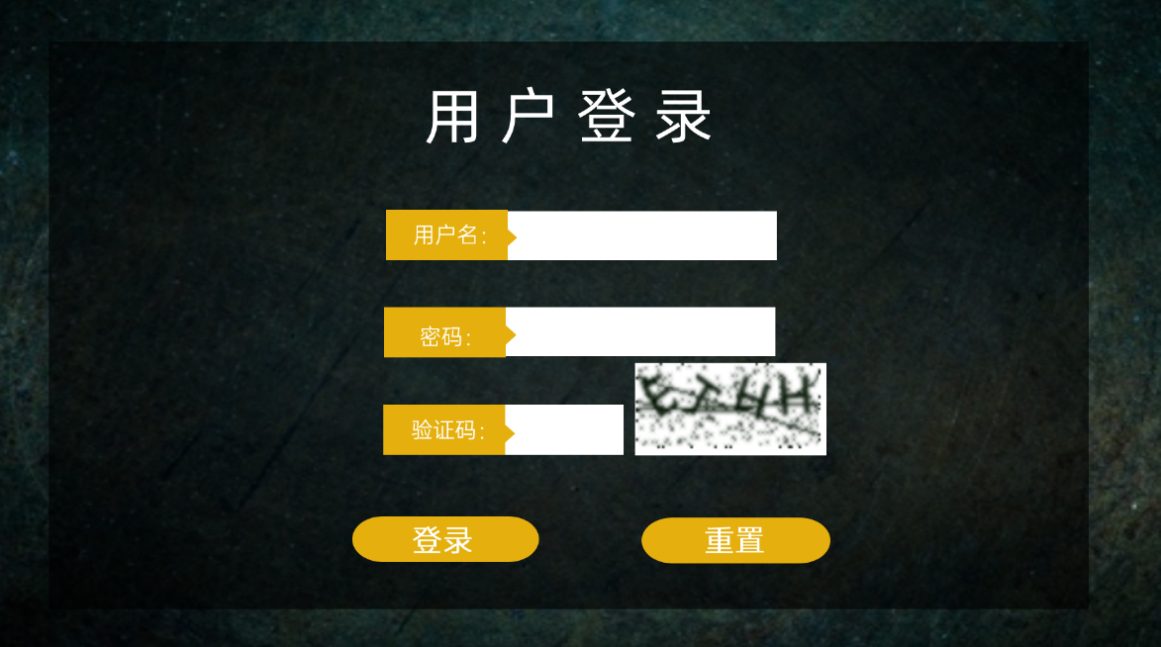
\includegraphics[width=\textwidth]{p2.png}
\caption{登录页面样式} % 标题
\label{five}
\end {figure}

\subsection{注册页面}
页面顶部为“用户注册”的标题,页面主体为register表单,注册信息主要包括用户名、密码、确认密码、性别和验证码。输入用户名和密码后,将输入的数据与后端数据库中的数据进行对比,若用户名已存在会提醒账号已注册;将密码和确认密码、输入验证码与随机验证码相对比,若不相同会提醒错误。账号未被注册且输入数据正确后将显示注册成功并回到登录页面。
\begin {figure}[h]
\centering % 居中显示
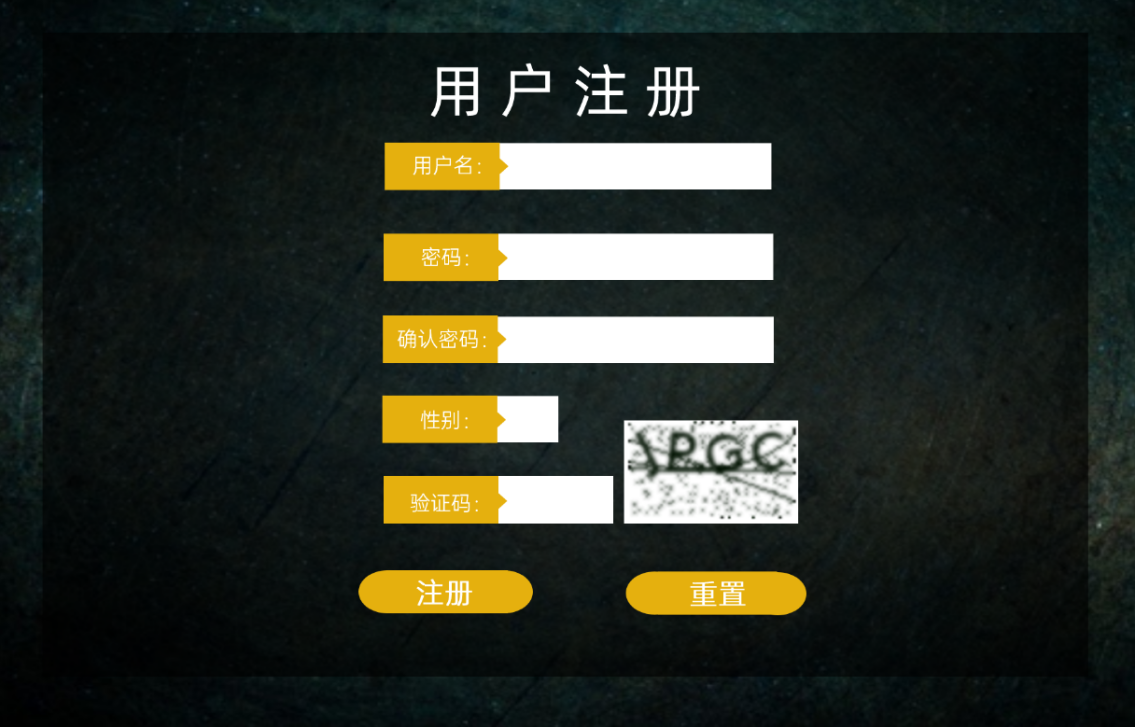
\includegraphics[width=\textwidth]{p3.png}
\caption{注册页面样式} % 标题
\label{five}
\end {figure}

\subsection{登陆首页}
登录后的主页的框架与未登录主页大致相同,在左侧电影分类目录中添加了“猜你喜欢”分栏,点击后页面呈现的电影资源为利用推荐算法,将电影综合评价得出的电影排序;顶部显示用户名,点击可进入个人信息页面。
\begin {figure}[h]
\centering % 居中显示
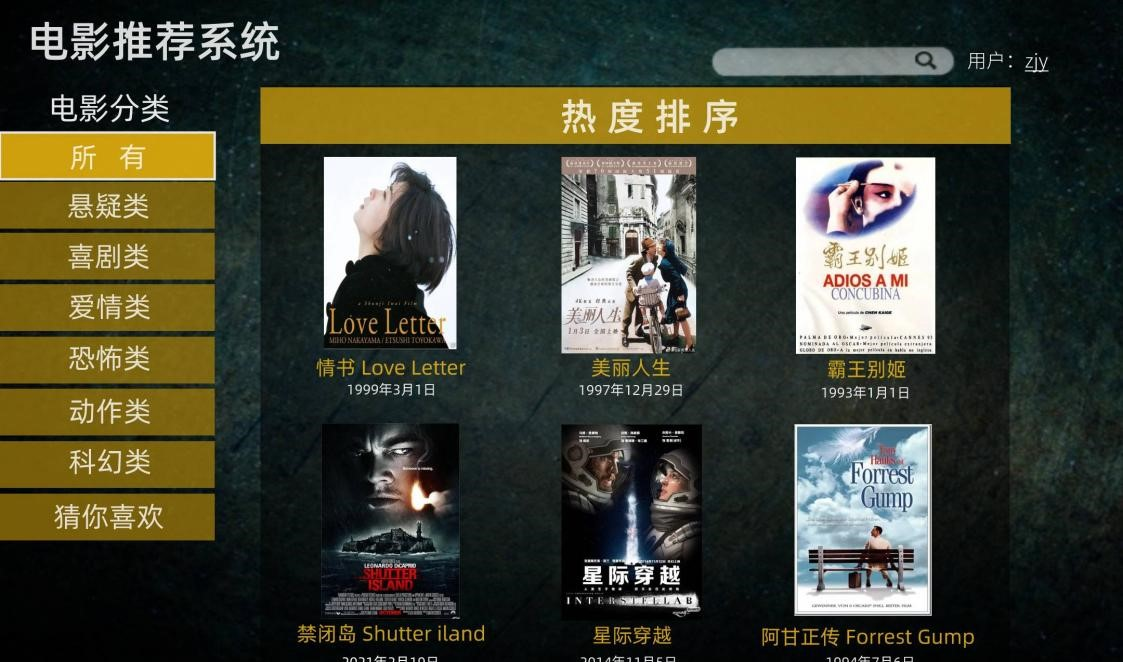
\includegraphics[width=\textwidth]{p4.jpg}
\caption{登录首页样式} % 标题

\label{five}
\end {figure}

\section{系统算法模型}

\subsection{基于图注意力的归纳式图嵌入推荐模型}

本文提出的基于图注意力的归纳式图嵌入推荐模型由以下几个部分组成:
\begin{enumerate}
    \item 封闭子图提取:不采用在原始图即原始邻接矩阵上操作的方式,而是对每个用户/项目对进行封闭子图提取。训练好的模型在每个子图上独立进行预测。
    \item RGAT注意力层:使用四层堆叠的RGAT图神经网络层进行节点特征表征。
    \item 池化层:将各层的隐向量拼接成为最终的子图表示。
    \item MLP全连接层:将子图嵌入作为输入预测评分值。
\end{enumerate}

\subsubsection{封闭子图提取}
第一部分是封闭子图提取。封闭子图指的是基于图原始邻接矩阵所提取的子图,即包括原始图部分节点的子图。我们使用$G$来表示由评分矩阵 构造而来的无向用户/项目二部图。在图$G$中,用户类型节点用$u$表示,项目类型节点用$v$来表示,该图中只存在用户与项目之间的连边,即用户$u$对项目$v$有过历史评分$r$,不存在用户与用户以及项目与项目之间的连边。对于观察到的某一用户$u$对某一项目$v$的评分$r=R_{u,v}$,我们从$G$中提取一个围绕$(u,v)$的一跳封闭子图。我们将提取到的一跳封闭子图馈送到GNN,利用已知的$(u,v)$对的评分训练GNN模型。然后,测试阶段对于每个测试$(u,v)$对,我们再次从$(u,v)$中提取其一跳封闭子图,并使用经过训练后的GNN模型预测其评分。需要注意的是,在提取$(u,v)$的训练封闭子图之后,我们应该在封闭子图中删除边$(u,v)$,因为它是要预测的目标。

\subsubsection{图注意力消息传递层RGAT}
这一部分是训练一个多层附加注意力机制的图神经网络模型。为了考虑到不同边类型以及使用注意力机制关注不同的邻居。我们采用RGAT作为GNN的消息传递层,并对其做改进成为多层网络堆叠形式,以提高网络对图特征的提取能力。同时进行多次实验测试选择合适的注意力系数运算方案来适应本课题的推荐任务。

\begin{itemize}
    \item 网络输入与输出:
    
    这里介绍每个消息传递层的输入与输出形式,输入到某神经网络层$l$的形式为一个具有$R = \mathfrak{R} $个边类型数量和总共$N$个节点的二部图。第$l$层的第$i$个节点被表示成一个特征向量 $\mathbf{x}_i^l\in\mathbb{R}^F$,全部节点的特征向量可以聚合表示为一个矩阵,即$\mathbf{X}^l=[\mathbf{x}_1^l\mathbf{x}_2^l\cdots \mathbf{x}_N^l]\in\mathbb{R}^{N*F}$。输出则是该层经过一系列变换后的矩阵$\mathbf{X}^{l+1}=[\mathbf{x}_1^{l+1}\mathbf{x}_2^{l+1}\cdots \mathbf{x}_N^{l+1}]\in\mathbb{R}^{N*F'}$其中 $\mathbf{x}_i^{l+1}\in\mathbb{R}^{F'}$是第$i$个节点初始特征在第 $l$层经过变换后的输出,即该神经网络层计算后的节点向量表征。

    \item 节点中间表征 :
    
    不同边类型$r$应该传递不同的信息,对应每种边类型$r$应使用相应可学习的权重矩阵进行一次中间特征变换,对于节点中间表征$d_i^{l(r)}$更新规则如下


    \begin{equation}
        \mathbf{D}^{l(r)}=\mathbf{X}^l\mathbf{W}^{l(r)}
    \label{}
    \end{equation}
​    
其中$\mathbf{X}^l$是第$l$层的输入矩阵,$\mathbf{W}^{l(r)}\in\mathbb{R}^{F*F'}$是第$l$层中特定边类型$r$的一个可学习的参数矩阵,$\mathbf{D}^{l(r)}=[\mathbf{d}_1^{l(r)}\mathbf{d}_2^{l(r)}\cdots \mathbf{d}_N^{l(r)}]\in\mathbb{R}^{F*F'}$是该层初始输入 $\mathbf{X}^l$在边类型 $r$下的经变换后的中间表征。该步骤主要是对于不同边类型 $r$的输入特征向量进行特征变换,获得在不同边类型 $r$下的节点特征向量。
    \item 节点关联度计算统一形式:
    
    节点关联度指的是两个节点的关联程度大小,作为节点之间注意力系数的中间计算形式,最后还需进行 softmax 函数归一化后获得最终的节点之间的注意力系数。在两个节点之间的节点关联度仅仅是基于这些节点的特征进行计算,只收集节点领域信息,该节点关联度不同于最终节点之间的注意力系数,节点关联度$E_{i,j}^{l(r)}$计算形式如下
\begin{equation}
    E_{i,j}^{l(r)}=a(\mathbf{x}_i^{l(r)},\mathbf{x}_j^{l(r)})
\end{equation}
  
其中$E_{i,j}^{l(r)}$对于每个边类型其中是独立的。其中 ,$j\in \eta_i^{(r)}$表示节点 $j$属于节点 $i$的邻域(即在用户/项目二部图中用户节点 $i$与项目节点 $j$有连边), 表示某种对于节点的节点关联度计算形式,在下面部分给出具体计算方法

    \item 查询向量$Q$,键向量$K$,权重值向量$V$:
    
    现我们给出节点关联度的具体形式表示:
    \begin{equation}
        q_i^{l(r)}=\mathbf{h}^{l(r)}_i\mathbf{Q}^{l(r)}\in\mathbb{R}
        \label{q}
    \end{equation}
    \begin{equation}
        k_i^{l(r)}=\mathbf{h}^{l(r)}_i\mathbf{K}^{l(r)}\in\mathbb{R}
        \label{k}
    \end{equation}

    

节点关联度计算需要由查询向量以及键向量计算得到,其中$\mathbf{Q}^{l(r)}\in\mathbb{R}^{F'}$为可学习的查询向量, $\mathbf{K}^{l(r)}\in\mathbb{R}^{F'}$为可学习的键向量,查询向量与键向量分别与$h_i^{l(r)}$做向量乘积,得到标量值$q_i^{l(r)}$与标量值$k_i^{l(r)}$作为节点的查询标量值与键标量值。

    \item 节点关联度具体计算:
    
    将节点$i$的查询标量与节点$j$的键标量值相加后,即表示这两个节点之间的匹配程度,用来描述$i$,$j$节点之间的关联程度大小,我们称之为节点关联度。

这里的节点关联度采用线性加和进行计算,也可以采取如乘积、拼接等方法计算得出节点$i$,$j$之间的关联度。

\begin{equation}
    E_{i,j}^{l(r)} = LeakyRelu(q_i^{l(r)}+k_i^{l(r)})
\end{equation}
,其中$LeakyRelu$函数具体形式如下:
\begin{equation}
    LeakyRelu(x)=\begin{cases}x,x>0 \\\\ \lambda x,x\leq 0\end{cases}
\end{equation}
,其中$\lambda$参数是预先设定的,在0到1的范围之内。
    \item 注意力系数: 
    
    采用跨关系传播机制,计算第 $l$层中边类型 $r$下节点 $i$与节点  $j$之间的注意力系数 $\alpha_{i,j}^{l(r)}$:
    \begin{equation}
        \alpha_{i,j}^{l(r)}=\frac{exp(E_{i,j}^{l(r)})}{\Sigma_{r'\in\mathfrak{R}}\Sigma_{k\in{\eta_{i}^{(r')}}}exp(E_{i,j}^{l(r')})},\forall i:\Sigma_{r\in\mathfrak{R}}\Sigma_{k\in{\eta_{i}^{(r)}}}\alpha_{i,j}^{l(r)}=1
        \label{al}
    \end{equation}

    此步骤计算方法为常使用的$softmax$函数,归一化计算节点$i$的邻域中某一特定节点对$(i,j)$之间的注意力系数大小
    \item 传播规则:
    
    给出最终的传播规则:
    % todo 标注序号
    \begin{equation}
        \mathbf{x}_i^{l+1}=\sigma(\Sigma_{r\in\mathfrak{R}}\Sigma_{j\in{\eta_{i}^{(r)}}}\alpha_{i,j}^{l(r)}\mathbf{h}_{j}^{l(r)})
    \end{equation}
    
    其中$h_j^{l(r)}$为出现在式(\ref{q},\ref{k})中的中间计算表示,$\alpha_{i,j}^{l(r)}$ 为式(\ref{al})计算的到的节点$i$,$j$之间的注意力系数, $\sigma$为非线性激活函数,这里我们选择使用$ReLu$函数

    \begin{equation}
        ReLu(x)=\begin{cases} x,x>0 \\\\ 0,x\leq 0 \end{cases}
    \end{equation}

\end{itemize}
\subsubsection{池化层}
将节点表示池化到整个封闭子图级别的特征向量中。常规的池化操作由求和、求平均、排序、DiffPooling等。我们使用将目标用户与目标项目的最终嵌入表示作拼接,增强节点特征的信息,作为子图的表示。

节点$i$的最终向量表示:
\begin{equation}
    \mathbf{h}_i=concat(\mathbf{x}_i^1,\mathbf{x}_i^2,\cdots,\mathbf{x}_i^l)
\end{equation}

然后,将处于同一封闭子图中的目标用户节点表征与目标项目节点表征做拼接池化成该子图的嵌入:
\begin{equation}
    \mathbf{g}=concat(\mathbf{h}_u,\mathbf{h}_v)
\end{equation}

我们使用$\mathbf{h}_u$ 与$\mathbf{h}_v$ 来分别表示最终的目标用户和目标项目,将$\mathbf{h}_u$ 与$\mathbf{h}_u$ 向量作拼接形成该子图的嵌入表示 $\mathbf{g}$。

\subsubsection{MLP全连接层}
使用两层全连接神经网络,维度形状分别为$[128,32]$以及$[32,1]$
\begin{equation}
    \hat{r}=\mathbf{w}^T\sigma(\mathbf{Wg})
\label{}
\end{equation}
其中$\mathbf{W}$ 和$\mathbf{w}$ 是MLP的参数,用来将图表征 $\mathbf{g}$转换为一个标量评分值$\hat{h}$ ,其中 $\sigma$为非线性激活函数,我们使用$ReLu$函数。
\subsection{模型训练}
我们设置最小化模型预测评分与数据集真实评分之间的均方根误差(MSE),作为损失函数,公式如下:
\begin{equation}
    \mathcal{L}=\frac{1}{\left|\left\{(u, v) \mid \Omega_{u, v}=1\right\}\right|_{(u, v): \Omega_{u,}, v}} \sum_{u, 1}\left(R_{u, v}-\widehat{R}_{u, v}\right)^{2}
\label{}
\end{equation}
\section{实验与分析}

\begin{table}[t]
    \centering
    \begin{tabular}{ccc}
    \toprule
    \multicolumn{1}{c}{\textit{训练轮数}}
      &&\multicolumn{1}{c}{\textit{误差}}  \\ \midrule
    1	&&0.970\\
    10	&&0.946\\
    20	&&0.922\\
    30	&&0.924\\
    40	&&0.920\\
    50	&&0.919\\
    60	&&0.912\\
    70	&&0.910\\
    80	&&0.910\\
    \bottomrule
      \end{tabular}
    \caption{模型训练结果}
    \label{tabula}
    \end{table}

在建立电影推荐模型之后,我们使用MovieLens-100K数据集进行模型的训练与评估。训练集与测试集占比分别为$90\%$与$10\%$。得到表\ref{tabula}的结果:

在80轮训练结束过后,模型误差下降至$RMSE=0.910717$,具有较好的效果。

\section{总结与展望}
\subsection{工作总结}

目前我们已完成本课题《基于图嵌入技术的推荐算法研究》的详细设计及代码编写。实施方案采用Python程序设计语言及相关工具库Pytorch、Pytorch\_Geometric等进行图卷积网络搭建。主要思路是先对数据集进行用户/项目一跳封闭子图的提取,在封闭子图上用考虑评分类型的图注意力神经网络模型训练后得到子图的嵌入表示,后将子图嵌入向量通过两层全连接神经网络计算得到用户对项目的预测评分值。

本实验过程中多次调整、变换网络结构,最终已达到较高的预测精度。代码已基本实现完成并经过在实机上的运行测试。

在完成了推荐训练模型设计后,我们还完善了以Django作为后端,以Bootstrap作为前端的电影推荐网页设计,完成了注册,登录,电影推荐,电影分类的基本功能,且在注册过程中使用了验证码防止恶意注册。我们还采用Scrapy进行数据挖掘工作,充实了电影数据来源。
\subsection{展望}
在数据挖掘方面,我们已经收集了一些数据,但是这远远不能满足需求,我们还需要收集更多电影数据。为此,我们将尽可能实现基于Scrapy的分布式搭建数据挖掘框架,并在此基础上结合redis数据库实现增量式爬虫来获取更多的数据。

在前后端不分离架构中,所有的静态资源和业务代码统一部署在同一台服务器上。服务器接收到浏览器的请求后,进行处理得到数据,然后将数据填充到静态页面中,最终返回给浏览器。而前后端分离的架构开发效率更高,用户访问速度更快,可减轻后端服务器的请求压力。
在后期工作中,我们将进行前后端分离的工作。主要解决方法是用Bootstrap+Vue前端页面调用后端接口。

在未来的工作中,我们还将添加实时推荐系统,以创建一个更加符合人们使用习惯的电影推荐系统。实施推荐系统将传统的T+1(按天)推荐调整为秒级推荐,带来了处理效率的极大提升。

该实时推荐系统分为三个步骤:
\begin{itemize}
    \item 实时获取
    \item 实时计算
    \item 实时更新
\end{itemize}

就架构而言,实时推荐系统具有下图\ref{post}所示的架构:

\begin {figure}[h]
\centering % 居中显示
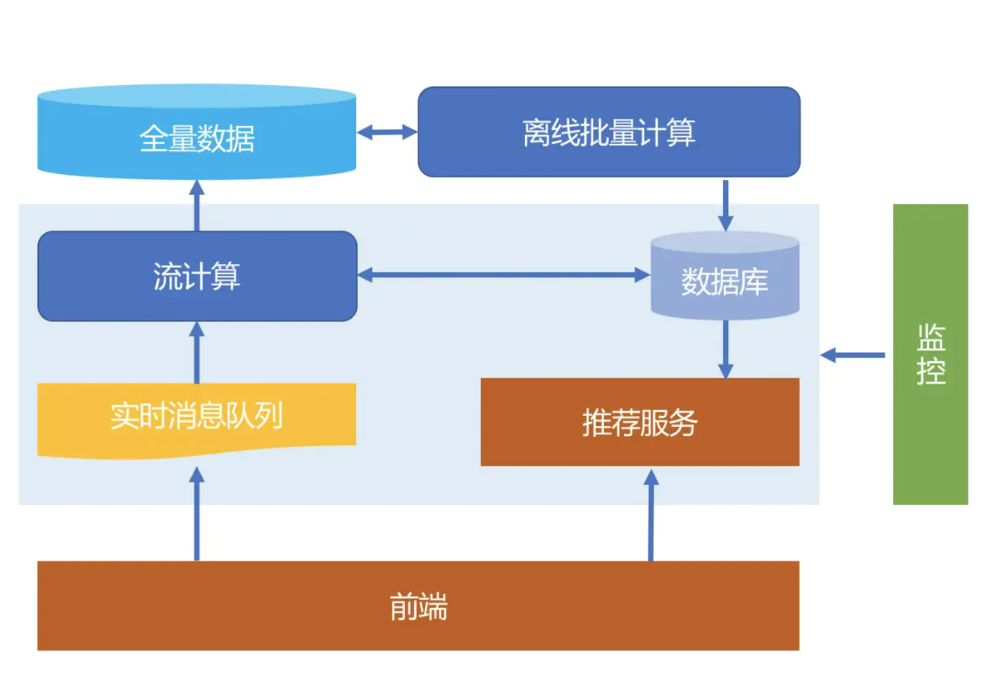
\includegraphics[width=0.7\textwidth]{post.png}
\caption{实施推荐系统结构图} % 标题
\label{post}
\end {figure}

经过调研,我们发现在实时推荐系统的算法实现中,目前主流的实施推荐算法有以下几种:
\begin{enumerate}
    \item 聚类技术和实时协同过滤算法
    \item 基于Spark方式
    \item 基于Kiji框架
    \item 基于Storm
\end{enumerate}

我们将在后期工作中完善实施推荐功能。
\end{document}
